\documentclass[aspectratio=169,xcolor=dvipsnames]{beamer}
\makeatletter
\def\input@path{{theme/}}
\makeatother
\usetheme{CleanEasy}
\usepackage{comment}
\usepackage[utf8]{inputenc}
\usepackage{lmodern}
\usepackage[T1]{fontenc}
% \usepackage[brazil]{babel}
\usepackage{fix-cm}
\usepackage{amsmath}
\usepackage{mathtools}
\usepackage{listings}
\usepackage{float}
\usepackage{caption}
\usepackage{subcaption}
\usepackage{xcolor}
\usepackage{hyperref}
\usepackage{graphicx} % Allows including images
\usepackage{booktabs} % Allows the use of \toprule, \midrule and \bottomrule in tables
\usepackage{tikz}
\usetikzlibrary{positioning, shapes, arrows, calc, decorations.pathreplacing, arrows.meta, backgrounds, patterns, overlay-beamer-styles}
\usepackage{etoolbox}
\usepackage{cancel}
% Opzionale: cambia il colore della sbarra in rosso per renderla più visibile
\renewcommand{\CancelColor}{\color{red}}
\usepackage{animate}
\usepackage{algorithmic}


%----------------------------------------------------------------------------------------
%    LAYOUT CONFIGURATION
%----------------------------------------------------------------------------------------

%----------------------------------------------------------------------------------------
%    TITLE PAGE
%----------------------------------------------------------------------------------------

%----------------------------------------------------------------------------------------



% Title Page Information
\title[Modeling Cellular Exhaustion]{Mathematical Models at the Population Level to Support Immunotherapy Design}
\author[Alibrandi Orazio]{Alibrandi Orazio}
\institute[Uni]{Department of Mathematics}
\date{May 28, 2026}

\begin{document}

% Slide 1: Title
\begin{frame}
    \titlepage
\end{frame}

% Slide 2: Contents
\begin{frame}{Contents}
    \tableofcontents
\end{frame}

% ---------------------------------------------------
\section{1. Immune System Functioning}
% ---------------------------------------------------

\begin{frame}{Immune System Functioning}

\begin{figure}
    \centering
    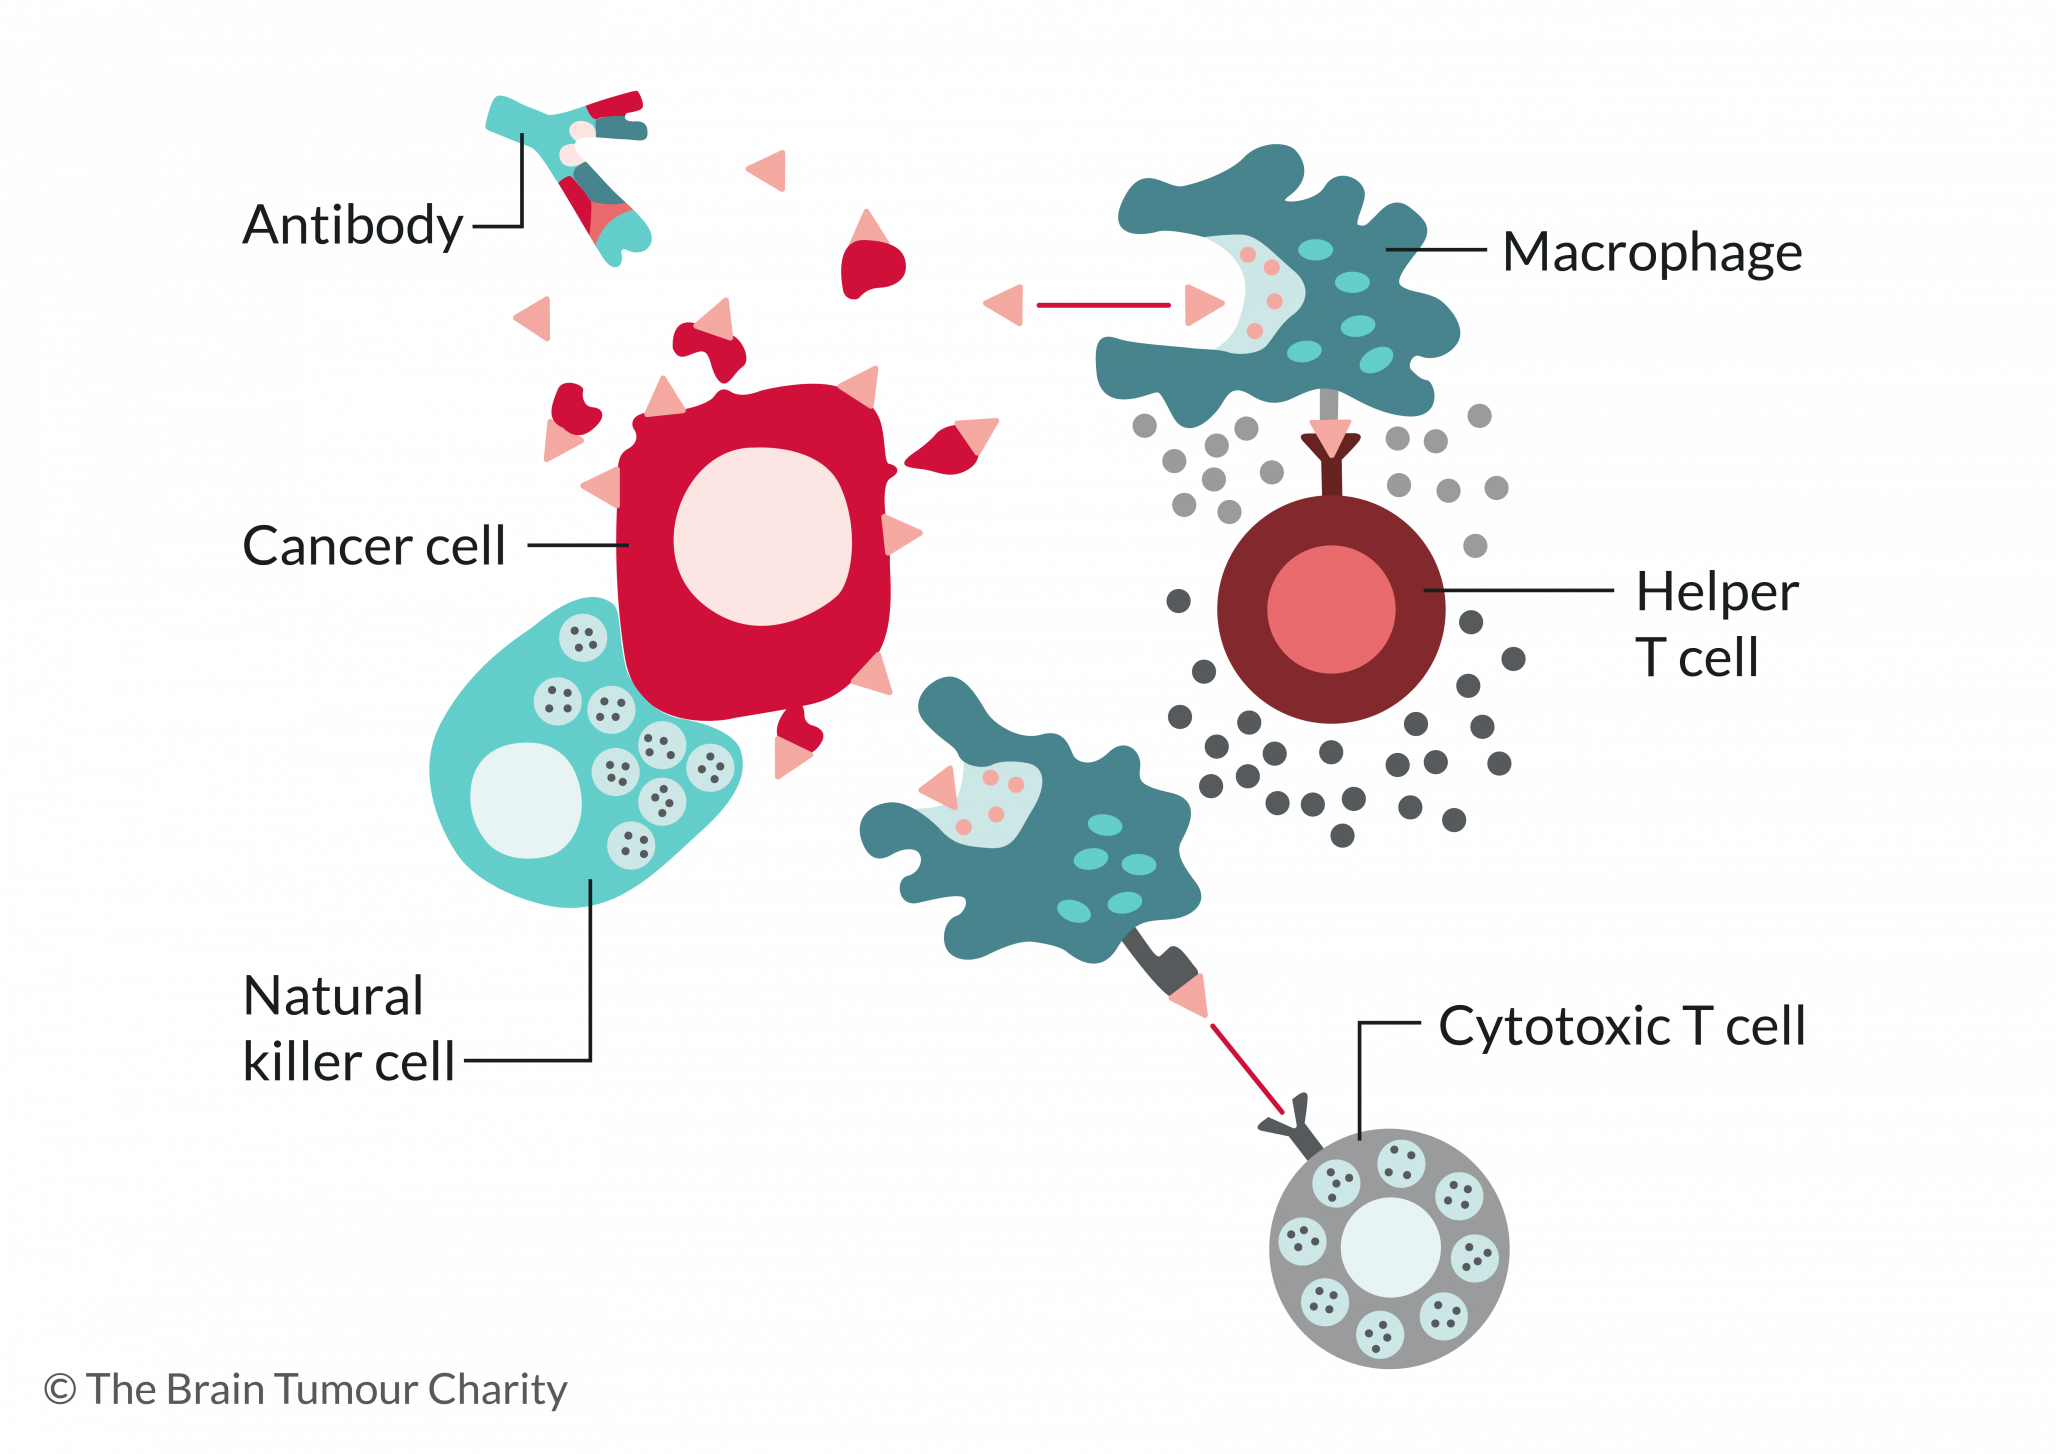
\includegraphics[width=0.6\textwidth]{../pics/immunesystem.png}
    \end{figure}
%     \begin{itemize}
%         \item The immune system plays a crucial role in defending the body against diseases, including cancer, by identifying and eliminating abnormal cells.
%         \item One of its most effective components are T cells, which recognize and attack malignant cells.
%         \item Naïve T cells differentiate into effector cells: CD4+ Helper T cells (coordinating via cytokines) and CD8+ Cytotoxic T cells (CTLs, actively killing the infection).
%         \item Under conditions of chronic stimulation such as persistent exposure to tumor-associated antigens, T cells can enter a dysfunctional phase called immune cell exhaustion.
%         \item Exhausted T cells become too weak to fully eliminate the threat, leading to a localized tumor-immune stalemate.
%     \end{itemize}
\end{frame}

% ---------------------------------------------------
\section{2. Formulation of the Model}
% ---------------------------------------------------

\begin{frame}{Foundational ODE Model}
    The model developed by Simmons and Levy \cite{SimmonsLevy} describes the development of cellular exhaustion. It uses five state variables:
    \vspace{0.2cm}
    \begin{itemize}
        \item $N$: Tumor volume.
        \item $K$: Residual healthy CTL (CD8+) population.
        \item $B$: Progenitor Exhausted T cells.
        \item $E$: Terminally Exhausted T cells.
        \item $P$: Interleukin-2 (IL-2) cytokine concentration.
    \end{itemize}
\end{frame}

\begin{frame}{ODE Model (Equations)}
    The dynamics of the system are described by the following set of ODEs:
    \begin{equation*}
        \begin{cases}
            \dot{N}(t) &= \alpha N \left(1 - \frac{N}{T_c}\right) - h \left( \frac{\lambda_K N K + \lambda_E N E}{N + K + E + 1} \right) \\
            \dot{K}(t) &= h P K - \delta_K K \\
            \dot{B}(t) &= 2^m s_B N + h P B - r_E B - \delta_B B \\
            \dot{E}(t) &= r_E B - \delta_E E \\
            \dot{P}(t) &= \rho_K K + \rho_B B - h P (K + B) - \delta_P P
        \end{cases}
    \end{equation*}
\end{frame}

\begin{frame}
    \begin{figure}
        \centering
        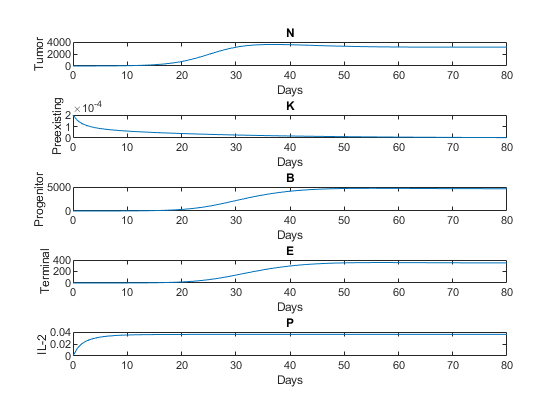
\includegraphics[width=0.7\textwidth]{../pics/Paper_model.png}
        \vspace{-0.3cm}
        \caption{Reproduction of the model dynamics showing the evolution of N ,
        K, B, E, and P over time.}
    \end{figure}
\end{frame}
% ---------------------------------------------------
\section{3. Extending the Model}
% ---------------------------------------------------

\begin{frame}{Extending the model: multiple exhaustion states}
    To capture the heterogeneity of T cell exhaustion, the $E$ group of cells has been divided following different levels of exhaustion:
    \begin{itemize}
        \item $E_0$: Initially Exhausted T cells (functional, capable of tumor killing).
        \item $E_{1/2}$: Middle-exhausted T cells (partially dysfunctional).
        \item $E_1$: Deeply-exhausted T cells (fully exhausted, negligible killing capabilities).
    \end{itemize}
    \vspace{0.2cm}
\end{frame}

\begin{frame}{ODE Model with Multiple Exhaustion States}
    The extended model is described by the following set of ODEs:
    \begin{equation}
\begin{cases}
    \dot{N}(t) = \alpha N \left(1 - \frac{N}{T_C}\right) - h \left( \frac{\lambda_k N K + \lambda_0 N E_0 + \lambda_{1/2} N E_{1/2} + \lambda_1 N E_1}{N + K + E_0 + E_{1/2} + E_1} \right), \\[2ex]
    \dot{K}(t) = h P K - \delta_k K, \\[2ex]
    \dot{B}(t) = 2^m S_B N + h P B - r_E B - \delta_B B, \\[2ex]
    \dot{E}_0(t) = r_E B - r_t E_0 - \delta_0 E_0, \\[2ex]
    \dot{E}_{1/2}(t) = r_t E_0 - r_t E_{1/2} - \delta_{1/2} E_{1/2}, \\[2ex]
    \dot{E}_1(t) = r_t E_{1/2} - \delta_1 E_1\\[2ex]
    \dot{P}(t) = \rho_K K + \rho_B B - h P (K + B) - \delta_P P,
\end{cases}
\end{equation}
\end{frame}

\begin{frame}{Homogeneity in killing and death rates}
    With the assumption of homogeneity in the death rates ($\delta_0 = \delta_{1/2} = \delta_1 = \delta_E$) and in the killing rates ($\lambda_0 = \lambda_{1/2} = \lambda_1 = \lambda_E$), we can recover the original equation for $E$:
    
    \vspace{0.3cm}
    \begin{equation*}
    \begin{aligned}
        \dot{E} &= \dot{E}_0 + \dot{E}_{1/2} + \dot{E}_1 
        \pause \\[1.5ex]
        % Usa \only per mostrare la riga pulita al passo 2, e quella sbarrata dal passo 3 in poi
        &= \only<2>{(r_E B - r_t E_0 - \delta_E E_0) + (r_t E_0 - r_t E_{1/2} - \delta_E E_{1/2}) + (r_t E_{1/2} - \delta_E E_1)}%
           \only<3->{(r_E B - \cancel{r_t E_0} - \delta_E E_0) + (\cancel{r_t E_0} - \cancel{r_t E_{1/2}} - \delta_E E_{1/2}) + (\cancel{r_t E_{1/2}} - \delta_E E_1)}
        \pause\pause \\[1.5ex] % Doppio pause per gestire lo sdoppiamento di sopra
                &= r_E B - \delta_E (E_0 + E_{1/2} + E_1) 
        \pause \\[1.5ex]
                &= r_E B - \delta_E E.
    \end{aligned}
    \end{equation*}
\end{frame}

\begin{frame}{Homogeneity in killing and death rates}
    In the same way, tumor equation is the same as the original one:
    \vspace{0.2cm}
    \begin{equation}
    \begin{aligned}
        \dot{N} &= \alpha N \left( 1 - \frac{N}{T_C} \right) - h \left( \frac{\lambda_k N K + \lambda_0 N E_0 + \lambda_{1/2} N E_{1/2} + \lambda_1 N E_1}{N + K + E_0 + E_{1/2} + E_1 + 1} \right) \\[1ex]
                &= \alpha N \left( 1 - \frac{N}{T_C} \right) - h \left( \frac{\lambda_k N K + \lambda_E N E_0 + \lambda_E N E_{1/2} + \lambda_E N E_1}{N + K + E_0 + E_{1/2} + E_1 + 1} \right) \\[1ex]
                &= \alpha N \left( 1 - \frac{N}{T_C} \right) - h \left( \frac{\lambda_k N K + \lambda_E N (E_0 + E_{1/2} + E_1)}{N + K + (E_0 + E_{1/2} + E_1) + 1} \right) \\[1ex]
                &= \alpha N \left( 1 - \frac{N}{T_C} \right) - h \left( \frac{\lambda_k N K + \lambda_E N E}{N + K + E + 1} \right)
    \end{aligned}
    \end{equation}
\end{frame}

\begin{frame}
    \begin{figure}
        \centering
        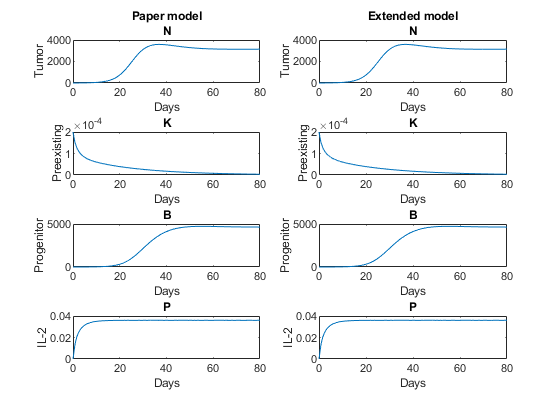
\includegraphics[width=0.7\textwidth]{../pics/PapervsNewHomo.png}
        \vspace{-0.3cm}
        \caption{Comparison between the original system and the new one.}
    \end{figure}
\end{frame}

\begin{frame}
    \begin{figure}
    \centering
    % PRIMA RIGA
    \begin{subfigure}[b]{0.49\textwidth}
        \centering
        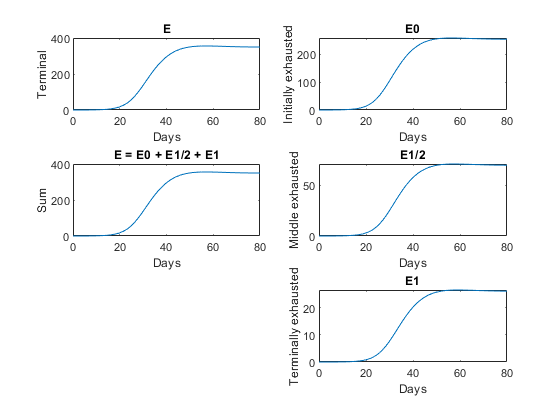
\includegraphics[width=1\textwidth]{../pics/E_sum_rt5.png} 
        
    \end{subfigure}
    \begin{subfigure}[b]{0.49\textwidth}
        \centering
        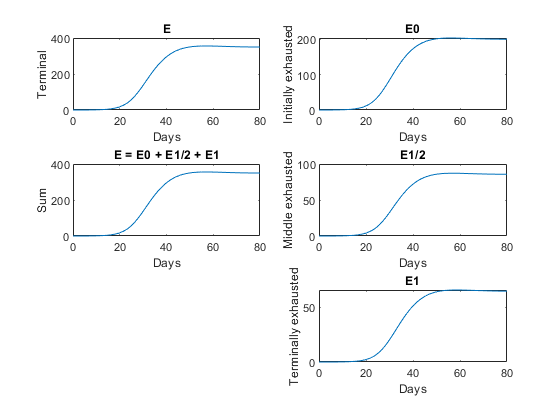
\includegraphics[width=1\textwidth]{../pics/E_sum_rt10.png}
    \end{subfigure}
    \caption{Comparison between the original system and the new one with $r_t=5r_E$ on the left and $r_t=10r_E$ to the right.}
\end{figure}
\end{frame}

\begin{frame}{Heterogeneity in killing and death rates}
    \begin{itemize}
        \item Deeper exhaustion is linked with a shorter lifespan:
        \begin{equation*}
            \delta_t(y) = \delta_{E_0} + (\delta_{E_1} - \delta_{E_0})y
        \end{equation*}
        \item Progressive exhaustion severly affects effector function:
        \begin{equation*}
            \delta_t(y) = \delta_{E_0} + (\delta_{E_1} - \delta_{E_0})y
        \end{equation*}
        \item T cells progressively pass from one state to the other in the following order:
        \begin{equation*}
            E_0 \rightarrow E_{1/2} \rightarrow E_1
        \end{equation*}
    \end{itemize}
\end{frame}

\begin{frame}
    \begin{figure}
    \centering
    % PRIMA RIGA
    \begin{subfigure}[b]{0.49\textwidth}
        \centering
        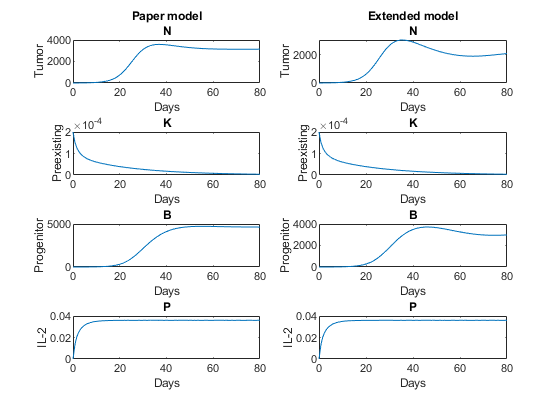
\includegraphics[width=1\textwidth]{../pics/PapervsNewHet.png} 
        
    \end{subfigure}
    \begin{subfigure}[b]{0.49\textwidth}
        \centering
        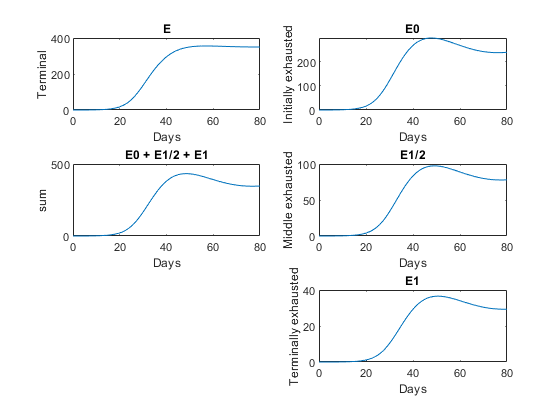
\includegraphics[width=1\textwidth]{../pics/E_sum_rt5_Het.png}
    \end{subfigure}
    \caption{Comparison between the original system and the new one with $r_t=5r_E$ and heterogeneous killing and death rates.}
    \end{figure}
\end{frame}

% ---------------------------------------------------
\section{4. Continuous Population Model}
% ---------------------------------------------------

% % Mimicking the step-by-step mathematical derivation slide from the ADAM example
% \begin{frame}{Derivation of the PDE Model}
%     Biological phenomena involving phenotypic variation can are more accurately modeled as continuous spectra
%     \vspace{0.2cm}
    
%     Let's consider a small piece of the space $\Delta y$ at time $t$.
%     \pause
    
%     The incremental number of cells in this piece is defined by advection and death:
%     \begin{equation*}
%         \frac{\partial}{\partial t}[E(t,y)\Delta y] = \nu(t,y)E(t,y) - \nu(t,y+\Delta y)E(t,y+\Delta y) - \delta_t(y)E(t,y)\Delta y
%     \end{equation*}
%     \pause
    
%     Dividing by $\Delta y$ we obtain the incremental ratio:
%     \begin{equation*}
%         \frac{\partial}{\partial t}E(t,y) = \frac{v(t,y)E(t,y) - v(t,y+\Delta y)E(t,y+\Delta y)}{\Delta y} - \delta_t(y)E(t,y)
%     \end{equation*}
%     \pause
    
%     Taking the limit $\Delta y \rightarrow 0$, we recognize an advection-reaction PDE:
%     \begin{equation*}
%         \frac{\partial}{\partial t}E(t,y) + \frac{\partial}{\partial y}(v(t,y)E(t,y)) = -\delta_t(y)E(t,y)
%     \end{equation*}
% \end{frame}

% \begin{frame}{Continuous Population Model (Summary)}
%     The final system is a coupled set of ODEs and a PDE.
%     \vspace{0.2cm}
%     \begin{itemize}
%         \item We introduce a continuous phenotype $y \in [0,1]$.
%         \item $E(t,y)$ represents the total number of exhausted cells at time $t$ characterized by phenotype $y$.
%         \item The boundary condition for the PDE represents the incoming flux of progenitor cells:
%     \end{itemize}
%     \begin{equation*}
%         v(t,0)E(t,0) = r_E B(t)
%     \end{equation*}
%     \begin{itemize}
%         \item The tumor-killing parameter $\lambda_t(y)$ and the death rate $\delta_t(y)$ are defined as continuous linear functions of $y$.
%     \end{itemize}
% \end{frame}

% \begin{frame}{Numerical Approach (Method of Lines)}
%     % Mimicking the pseudocode/algorithm block style
%     To numerically solve the coupled system of ODEs and PDEs, we used the Method of Lines (MOL).
    
%     \vspace{0.2cm}
%     \textbf{Discretization algorithm steps:}
%     \hrule
%     \vspace{0.1cm}
%     \begin{algorithmic}
%         \STATE \textbf{Initialize:} Partition domain $y \in [0,1]$ into $r = 1001$ nodes with step $h$.
%         \STATE \textbf{Advection:} Use a first-order backward finite difference approximation (upwind scheme) because cells travel in only one direction.
%         \STATE \textbf{Update Rule:} $\frac{d}{dt}E_i = \frac{v_{i-1}E_{i-1} - v_i E_i}{h} - \delta_i E_i$
%         \STATE \textbf{Boundary:} Apply $v(t,0)E(t,0) = r_E B(t)$ to the first grid point.
%         \STATE \textbf{Jacobian Assembly:} Build sparse matrix $J = [A_{ODE}; A_{PDE}]$ to handle severe stiffness.
%         \STATE \textbf{Solve:} Integrate using MATLAB's \texttt{ode15s}.
%     \end{algorithmic}
%     \vspace{0.1cm}
%     \hrule
% \end{frame}

% \begin{frame}{Results and Evolution}
%     \begin{columns}[T]
%         \begin{column}{0.5\textwidth}
%             % Left column: Text
%             \textbf{System Dynamics:}
%             \begin{itemize}
%                 \item The early exhausted cells ($E_0$) provide a strong, immediate killing power.
%                 \item This causes a sharp drop in tumor size.
%                 \item However, a smaller tumor means less antigen stimulation, cutting off the immune system's supply of Progenitor cells ($B$).
%                 \item This causes a permanent tumor-immune stalemate.
%             \end{itemize}
%         \end{column}
        
%         \begin{column}{0.5\textwidth}
%             % Right column: Image placeholder
%             \begin{figure}
%                 \centering
%                 \framebox[\textwidth]{\rule{0pt}{4cm} Insert Figure 6 Here}
%                 \caption{Evolution of variables under heterogeneous assumptions.}
%             \end{figure}
%         \end{column}
%     \end{columns}
% \end{frame}

% % ---------------------------------------------------
% \section{6. Conclusions}
% % ---------------------------------------------------

% \begin{frame}{Conclusions}
%     \begin{itemize}
%         \item Having more functional cells ($E_0$) clears the tumor faster. 
%         \item However, by removing the constant antigen stimulation, the immune system cuts off its own supply of T cells, resulting in a permanent stalemate.
%         \item Biological phenomena involving phenotypic variation can often be more accurately modeled as continuous spectra.
%         \item Using the Method of Lines with an upwind scheme and an analytical Jacobian efficiently resolves the stiffness of the resulting PDE-ODE coupled system.
%     \end{itemize}
% \end{frame}

% \begin{frame}[allowframebreaks]{References}
%     % Il comando \nocite{*} dice a LaTeX di includere tutte le voci presenti nel file .bib, anche se non sono state citate nel testo
%     \nocite{*} 
    
%     % Scegli lo stile della bibliografia (es. plain, unsrt, alpha, ieeetr)
%     \bibliographystyle{unsrt} 
    
%     % Inserisci il nome del tuo file .bib (senza l'estensione .bib)
%     \bibliography{../ref} 
% \end{frame}

\end{document}